%------------------------------------------%
%
% Cannabis Data Science #59
%
% Date: 3/30/2022
%
%------------------------------------------%
\documentclass[xcolor={dvipsnames}]{beamer}
\hypersetup{pdfpagemode = FullScreen}
\mode<presentation>{
  \usetheme{Boadilla}
  \usecolortheme{orchid}
  \usefonttheme{default}
  \setbeamertemplate{navigation symbols}{}
  \setbeamertemplate{caption}[numbered]
}
\setbeamersize{
  text margin left = 0.5in,
  text margin right = 0.5in
}

%------------------------------------------%
% Title
%------------------------------------------%
\title[\textbf{Cannabis Data Science \#59}]{}
\author{Cannabis Data Science}
\institute[]{\Large Cannabis Data Science \#59}
\date{March \nth{30}, 2022}

%------------------------------------------%
% Packages
%------------------------------------------%
\usepackage[english]{babel}
\usepackage[utf8x]{inputenc}
\usepackage{tikz} % For styling.
\usepackage{xparse}

%------------------------------------------%
% Colors
%------------------------------------------%
\definecolor{Green}{RGB}{34, 153, 84}
\definecolor{LightGreen}{RGB}{218, 247, 166}
\definecolor{DarkGreen}{RGB}{2, 48, 32}
\definecolor{Orange}{RGB}{255, 87, 51}
\definecolor{DarkOrange}{RGB}{199, 0, 57}
\definecolor{Yellow}{RGB}{255, 195, 0}

%------------------------------------------%
% Theme
%------------------------------------------%
\setbeamercolor*{palette primary}{bg=LightGreen, fg=DarkGreen}
\setbeamercolor*{palette secondary}{bg=LightGreen, fg=DarkGreen}
\setbeamercolor*{palette tertiary}{bg=LightGreen, fg=DarkGreen}

%------------------------------------------%
% Packages
%------------------------------------------%
\usepackage{amsmath}
\renewcommand*\footnoterule{} % No separating line on footnote.
\usepackage{mathtools} % For annotating equations.
\usepackage{hhline} % for double bars.
\usepackage[super]{nth} % For formatting 1st, 2nd, 3rd, etc.
\usepackage{graphicx, caption, subcaption}
\usepackage{setspace}

%------------------------------------------%
% Commands
%------------------------------------------%

% Top space.
\newcommand\T{\rule{0pt}{2.5ex}}

% Bottom space.
\newcommand\B{\rule[-1.25ex]{0pt}{0pt}}

% Blocks.
\newenvironment<>{Block}[2][.9\textwidth]
  {\setlength{\textwidth}{#1}
  \begin{actionenv}#3
    \def\insertblocktitle{#2}\par
    \usebeamertemplate{block begin}}
  {\par\usebeamertemplate{block end}
  \end{actionenv}}

% Balls.
\defbeamertemplate{enumerate item}{largeball}
{\begin{pgfpicture}{-1ex}{-0.65ex}{1.5ex}{1.5ex}
\usebeamercolor[fg]{item projected}
{\pgftransformscale{2.5}\pgftext{\Large\pgfuseshading{bigsphere}}}
{\pgftransformshift{\pgfpoint{0pt}{0.5pt}}
\pgftext{\usebeamerfont*{item projected}\small\insertenumlabel}}
\end{pgfpicture}}

% Fancy arrows.
\NewDocumentCommand\UpArrow{O{2.0ex} O{black}}{%
   \mathrel{\tikz[baseline] \draw [->, line width=0.5pt, #2] (0,0) -- ++(0,#1);}} % Fancy up-arrow.
\NewDocumentCommand\DownArrow{O{2.0ex} O{black}}{%
   \mathrel{\tikz[baseline] \draw [<-, line width=0.5pt, #2] (0,0) -- ++(0,#1);}} % Fancy down-arrow.

% Equations with numbers on the left.
\makeatletter
\newcommand{\LeftEqNo}{\let\veqno\@@leqno}
\makeatother

%------------------------------------------%
%
% Presentation
%
%------------------------------------------%
\begin{document}

% Title page.
\begin{frame}{}
  
\includegraphics[scale=0.33]{images/logo.pdf}
  \vspace*{-2\baselineskip}
  \titlepage

  % TODO: Add flare to title page?
  % Background
%\tikz[remember picture, overlay]
%\node[opacity=1.0, inner sep=0pt] at (current page.center){
%  
\includegraphics[width=\paperwidth, height=\paperheight]{images/cover.pdf}
%};  
  
\end{frame}

%------------------------------------------%
% History of Data Science
%------------------------------------------%

\begin{frame}{Looking back at the history of computing...}

\begin{figure}
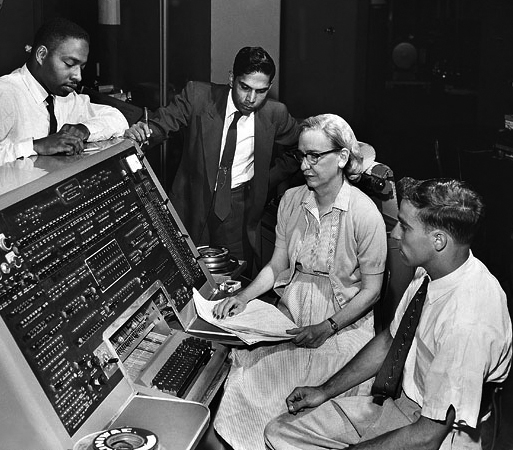
\includegraphics[width=0.9\textwidth]{images/grace-hopper-univac.jpg}
\end{figure}

\end{frame}


%------------------------------------------%
\begin{frame}{The Importance of Computers}

\vspace{0.5\baselineskip}

\begin{minipage}{0.6\textwidth}

\scriptsize

\vspace{0.5\baselineskip}

\begin{itemize}

\item Mathematician {\bfseries Grace Hopper} (``Grandma COBOL'') completes A-0, a program that allows a computer user to use \underline{English-like words} instead of numbers to give the computer instructions in 1952.

\vspace{0.25\baselineskip}

\item Helped the first commercial electronic computer and applications for COBOL (common-business-oriented language).

\vspace{0.25\baselineskip}

\item 70 years later, Google's fourth undersea internet cable, named Grace Hopper, connecting the US, UK, Spain, and is expected to soon be operational (2022).

\end{itemize}

\begin{figure}
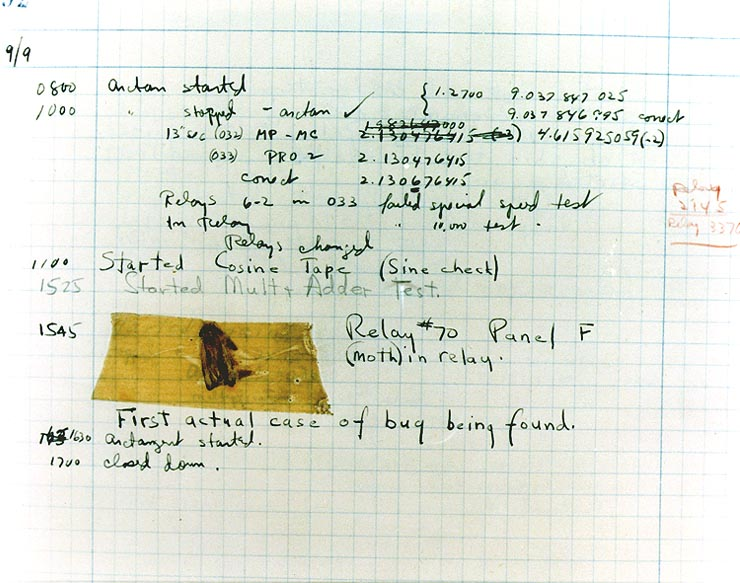
\includegraphics[width=1in]{images/first-computer-bug-1945.jpg}
\caption*{\tiny
First actual case of a bug being found (1960).\\
\tiny\color{Gray}
Author: Jan Arkesteijn
License: CC BY 2.0
https://creativecommons.org/licenses/by/2.0
}
\end{figure}

\end{minipage}\hspace{0.05\textwidth}%
\begin{minipage}{0.345\textwidth}

\begin{figure}
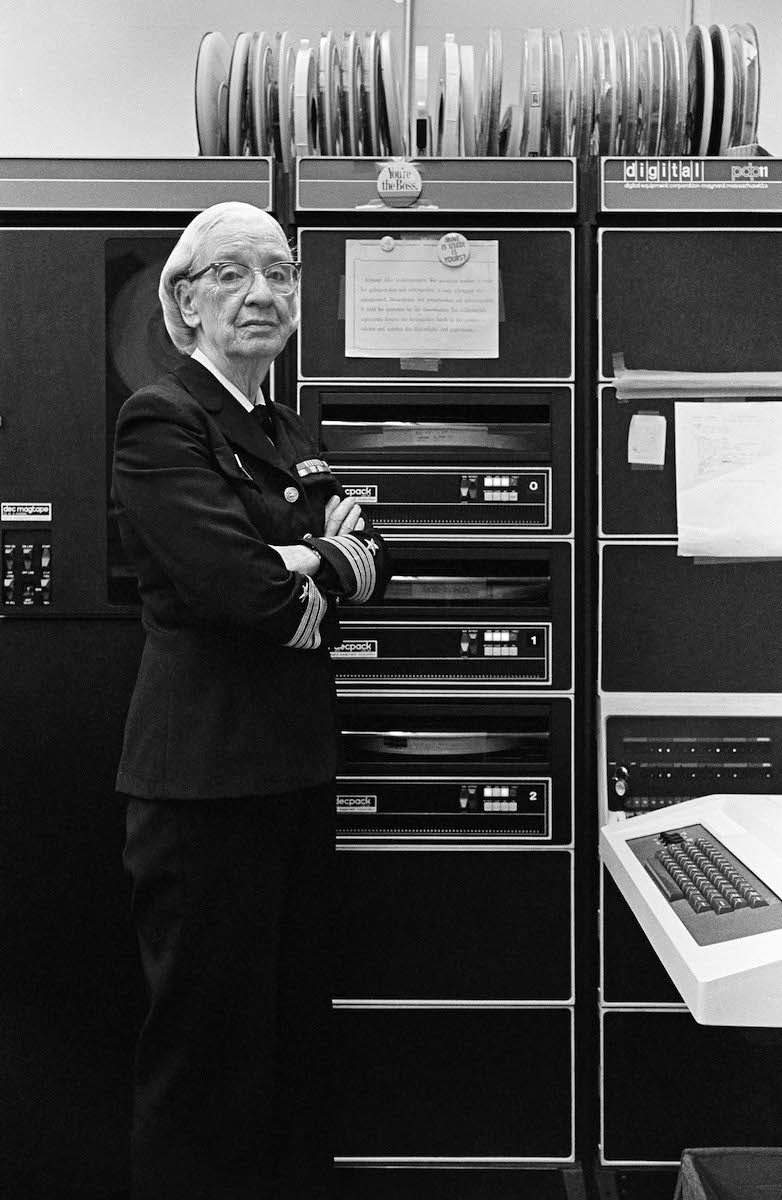
\includegraphics[width=\textwidth]{images/grace-hopper-computer.jpg}
\caption*{\setstretch{.75}{\tiny Grace Hopper, Washington DC, 1978.}\\[0.5\baselineskip]
{\setstretch{.75}\tiny\color{Gray} Author: Lynn Gilbert\\
License: CC BY-SA 4.0\\
creativecommons.org/licenses/by-sa/4.0}
}
\end{figure}

\end{minipage}

\end{frame}

%------------------------------------------%

\begin{frame}{From Top Secret to Open Access}

\begin{minipage}{0.5\textwidth}

\begin{figure}
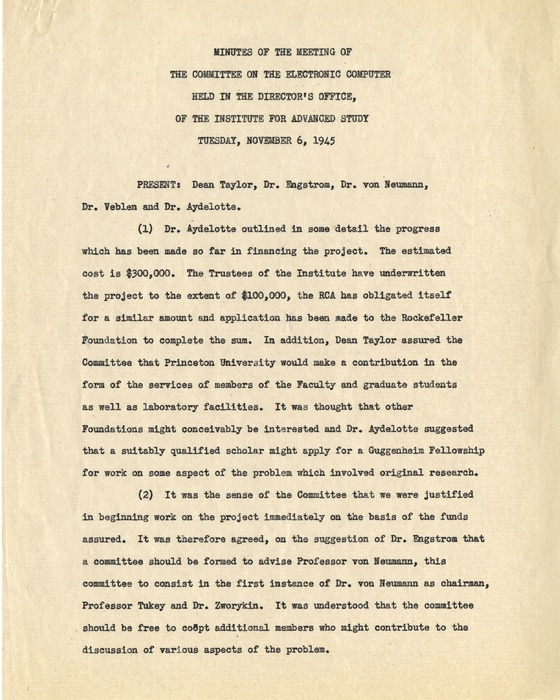
\includegraphics[height=0.75\paperheight]{images/minutes-1945.jpg}
\end{figure}

\end{minipage}\hspace{0.1\textwidth}%
\begin{minipage}{0.4\textwidth}

\small

The Electronic Computer Project (1945-1947)

\vspace{0.25\baselineskip}
\begin{itemize}

\item Led by Professor John von Neumann.

\vspace{0.125\baselineskip}

\item Put into the public domain.

\vspace{0.125\baselineskip}

\item 20,000,000 multiplications took 6 hours of continuous computing.

\end{itemize}

\end{minipage}

\end{frame}

%------------------------------------------%
\begin{frame}

\vspace{0.5\baselineskip}

{\itshape ``There are two kinds of people in the world:\\ Johnny von Neumann ...''}

\begin{figure}
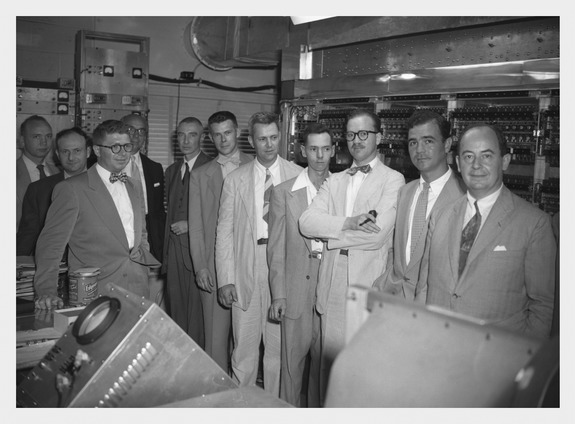
\includegraphics[width=\textwidth]{images/john-von-neumann-team.jpg}
\end{figure}

\end{frame}

\begin{frame}

\begin{figure}
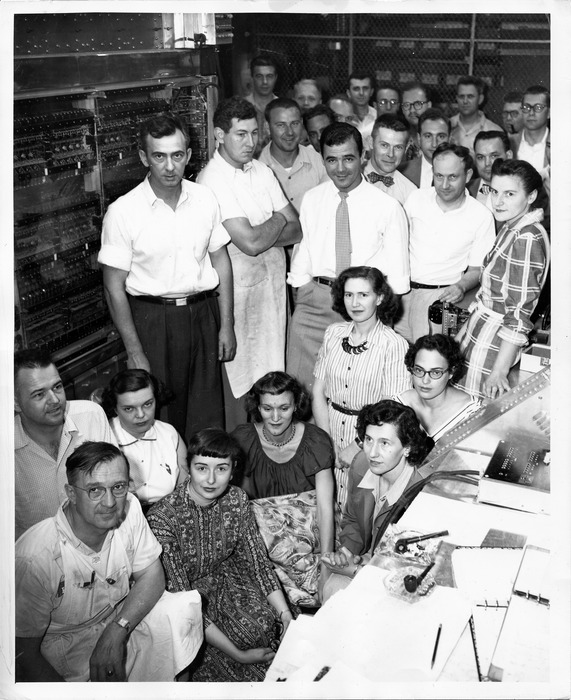
\includegraphics[width=0.65\paperheight]{images/computer-team.jpg}
\end{figure}

\begin{flushright}
{\itshape``...and the rest of us.''}

\vspace{0.125\baselineskip}
- Eugene Wigner
\end{flushright}

\end{frame}

%Source: Institute for Advanced Study
%------------------------------------------%


\begin{frame}{Searching for the origins of data science}

John von Neumann founded the field of {\bfseries game theory}.

\vspace{0.5\baselineskip}

\begin{itemize}

\item {\itshape Theory of Games and Economic Behavior},\\ von Neumann and Morgenstern (1944).

\vspace{0.25\baselineskip}

\item von Neumann–-Morgenstern utility function:

\vspace{-0.25\baselineskip}
$$
U(p) = \sum_{k=1}^K u(x_k)p_k
$$

where $p_{k}$ is the probability of outcome $k$ that, if realized, provides payoff $x_k$, and function $u$ expresses the utility of each respective payoff.

\vspace{0.25\baselineskip}

\item Today, {\bfseries Bayes' Theorem} is used to  endogenized probability, making it subjective. Subjective probabilities are updated in light of new information, thus connecting the concepts of {\bfseries rational choice} and inference.

\end{itemize}

\end{frame}


%------------------------------------------%
% A Sprinkle of Economics (excluded for time?)
%------------------------------------------%
%\section{A Brief Sprinkle of Economics}
%\begin{frame}{A Sprinkle of Economics: Competing for Profits}
%
%\vspace*{0.125\baselineskip}
%
%Market Effects
%
%- Michael Porter
%
%Competitive rivalry
%
%  - Degree of advertising
%  - Competitive Advantage / Comparative Advantage
%
%Buyer power
%
%  - Buyer concentration to firm concentration ratio
%  - Price elasticity of demand.
%
%Supplier power
%
%  - Input costs
%
%Threat of new entry
%
%Threat of substitution
%
%Observe:
%
%Markets of substitute goods tend to experience great volatility in prices, driving down producer profits.
%
%Prices tend to be reduced in attempts of producers to capture market share.
%
%Consumers may be able to attain more utility when there are available substitute products.
%
%In interdependent markets, game theory must be used to derive a profit maximizing solution.
%
%%\begin{itemize}
%%
%%\item Cournot
%%
%%\item Joseph Bertrand
%%
%%\item Pareto
%%
%%\item Irving Fisher
%%
%%\end{itemize}
%
%\end{frame}

% TODO: Talk about sbustitutes in production.


% TODO: Correlate concentration ratio for various product types and the vendors total sales (hue by producer type).

% that can produce cannabis products as {\bfseries substitutes in production}


%------------------------------------------%
% Game Theory
%------------------------------------------%
\section{Jumping into Game Theory}
\begin{frame}{Jumping into Game Theory}

\vspace*{0.125\baselineskip}

Repeated Games

\vspace*{0.5\baselineskip}
\begin{itemize}

\item {\bfseries Finite games}: Usually solved by backwards induction.

\vspace*{0.25\baselineskip}

\item {\bfseries Infinite games}: Typically, difficult to solve.

\vspace*{0.25\baselineskip}

\item Even if the game being played in each round is identical, repeating that game a finite or an infinite number of times can, in general, lead to very different outcomes (equilibria), as well as very different optimal strategies.

\end{itemize}

\end{frame}


\begin{frame}{Modeling Player Preferences}

Given that player $i$'s valuation of the game diminishes with time depending on a {\bfseries discount factor} $\delta < 1$, then player $i$'s utility is

$$
U_i = \sum_{t \geq 0}\delta^t u_i(x_t)
$$

where

$$
u_i(x_t) = \sum_{k=1}^K u_i(x_k)p_k
$$

\vspace{0.5\baselineskip}
The cutting edge is repeated games with incomplete information, where players have to formulate beliefs about probabilities, $p$.

\end{frame}


\begin{frame}{Solving Games}


{\bfseries Nash Equilibrium} -- A strategy profile for a game in which no player has a profitable unilateral deviation.


\vspace{2\baselineskip}

{\bfseries Subgame Perfect Nash Equilibrium} -- A strategy profile for a dynamic game with Nash equilibrium for every subgame.


\vspace{2\baselineskip}

{\bfseries Bayesian Nash Equilibrium} -- A strategy profile that maximizes the expected payoff for each player given their beliefs and given the strategies played by the other players.

%Every player's strategy maximizes their expected payoff given their beliefs about the state of nature.

\end{frame}


%------------------------------------------%
% Congestion Model
%------------------------------------------%
\section{Congestion Game}
\begin{frame}{Congestion Model}

\footnotesize

% TODO: Model product type production as a congestion game.

\vspace{0.5\baselineskip}
Given

\begin{itemize}

\item Cannabis {\color{RedOrange}producers}, $i = 1,...,N$,
\item Cannabis {\color{ForestGreen}products}, $m=1,...,M$,
\item A time horizon, $t=1,...,T$.

\end{itemize}

\vspace{0.75\baselineskip}
Under the following assumptions:

\begin{itemize}

\item Any {\color{RedOrange}producer} can produce any {\color{ForestGreen}product}.

\item The {\itshape cost} to produce an item of any type is $c=0$.

\item A {\color{RedOrange}producer} can change the type of {\color{ForestGreen}product} it produces at a set {\itshape interval}, $t_i$.\footnote{\tiny\itshape ``The Calvo Fairy is a mythical creature who arrives according to a Poisson process (i.e. inter-arrival times are exponentially-distributed).'' -Anonymous Economist}

\end{itemize}

\vspace{0.75\baselineskip}
{\bfseries Strategy}: Every time, $t_i$, a {\color{RedOrange}producer} can choose it's {\color{ForestGreen}product} type:

\vspace{0.25\baselineskip}
\begin{enumerate}

\item The {\color{RedOrange}producer} looks at the number of {\color{RedOrange}producers} of each type, $n_m$,

\vspace{0.25\baselineskip}

\item The {\color{RedOrange}producer} calculates the average profits for the {\color{RedOrange}producer} of each {\color{ForestGreen}product} type, $E[\pi]_m$, for $t_i$,

\vspace{0.25\baselineskip}

\item The {\color{RedOrange}producer} chooses the most profitable {\color{ForestGreen}product} to produce, $m*$, for $t_i$, taking into consideration that each other {\color{RedOrange}producer}, $j=1,...,J$, will produce the product that is most profitable for them at each $t_j$.

%enter or exit each product market depending on their best strategy at each $t_j$.
\end{enumerate}

\end{frame}


%\begin{itemize}
%
%\item It is easier to argue that there is natural variance in products such as flower, however, the ability for a beverage manufacturer to capture a large section of the market given a uniform product, typically a 100mg beverage, may depend largely on their marketing effectiveness.
%
%\item Do encumbants get market share?
%
%\item Run the gamut with beverage brand analysis.
%
%\item Using beverage product type for simplicity. The analysis can be readily applied to all product types.
%
%\end{itemize}


%------------------------------------------%
% Question and Hypothesis
%------------------------------------------%
\section{Question and Hypothesis}
\begin{frame}{Question and Hypothesis}

% Question of the day
\begin{center}
\begin{minipage}{.9\linewidth}
\begin{Block}{Question of the day.}

\vspace{.5\baselineskip}
\begin{itemize}

\item What is the {\bfseries Nash Equilibrium} of the congestion game?

\end{itemize}

\vspace{.5\baselineskip}

\end{Block}
\end{minipage}
\end{center}

\end{frame}


%------------------------------------------%
% Takeaway
%------------------------------------------%
\section{Takeaway}
\begin{frame}{}

\begin{center}
\begin{minipage}{3.85in}

% Thank you.

\includegraphics[width=.25in]{images/prayer.png} {\Large \textbf{Thank you for coming.}}\\[-0.5\baselineskip]

\begin{center}
\begin{minipage}{.9\linewidth}
\begin{Block}{Insight of the Day}

\vspace{0.5\baselineskip}

\begin{itemize}

\item It's all fun and {\bfseries games}, until someone makes a profit!

\vspace{0.5\baselineskip}

\end{itemize}

\end{Block}
\end{minipage}
\end{center}

\vfill

\end{minipage}
\end{center}

\vspace{0.5\baselineskip}

What would you like to talk about next week?

\vspace{0.5\baselineskip}

\end{frame}


%------------------------------------------%
% Fin.
%------------------------------------------%
\end{document}
